% !TeX encoding = UTF-8
% !TeX program = pdflatex

\documentclass[11pt]{article}
\usepackage{graphicx}
\usepackage{verbatim}

\newcommand\CIPH{C\!I\!P\!H_K}

\title{{\bf Practicing with an offline dictionary attack} \\ \bigskip \large HW2 - CNS Sapienza}
\date{2019-11-14}
\author{Valerio Coretti 1635747}
\pagenumbering{roman}

\begin{document}
\maketitle

\section{Introduction}
When we have to encrypt a file we always must be sure that our key was very strong, because nowadays there are many techniques to defeating a cipher.

However in the most of cases many people have a tendency to choose very simple passwords that are common words or slightly different variants of these, for example string that are obtained by appending a number or a punctuation character.

This type of passwords are vulnerable to a known attack called: {\em Dictionary Attack}.

A Dictionary attack is a {\em brute-force attack}, this means that it tries all the strings in a pre-arranged listing, typically derived from a list of words, such as a dictionary. Then a dictionary attack is not a real brute force attack, where a large proportion of the key space is searched systematically, but it tries only the string in the dictionary.

There are two types of Dicitionary attack: {\em Offline Dictionary Attack} and {\em Online Dictionary Attack}. The first working offline and eliminates all network related limitations to password guessing. In fact, it looks for all the possibilities in a file stored in the file system. Instead in an online attack, a hacker uses the same interface as a regular user to try to gain access to accounts. In both types all the attacker needs is a curated list of likely passwords.

In our project we have a ciphertext that has been encrypted with a definite command that we know:

\bigskip
$ openssl\;enc\;-e\;-aes-192-cbc\;-pbkdf2\;-in\;infile\;-out\;ciphertext $
\bigskip

Our goal is, appling the opposite command for every words in the chosen dictionary, to find the right password and relatively plaintext. Then we should simulate the command:

\bigskip
$ openssl\;enc\;-d\;-aes-192-cbc\;-pbkdf2\;-in\;ciphertext\;-out\;plaintext $
\bigskip

In the following sections we will see a simplify implementation of an offline dictionary attack in C code using OpenSSL Open-Source library, with Linux Mint and over an Intel core i5 64bit processor with 4GB of RAM.

\section{Preliminary Settings}
Being a brute-force attack if we don't say anything about what we want to decrypt and how it has been encrypted, it is very hard to attack it. But luckily in our case we have precise preliminary data given by the command above. Analyze it:

\begin{itemize}
\item {\em "openssl enc -e"}: invokes the openssl tool to encrypt and decrypt files, in our case -e indicates that we are encrypting a file.
\item {\em "-aes-192-cbc"}: indicates that to perform encryption we are using the AES algorithm with CBC operating mode and 192 key bits.
\item {\em "-pbkdf2"}: algorithm that derives a key from the input password (see the following section)
\item {\em "-in"} e {\em "-out"}: input file to encrypt and output file for ciphertext
\end{itemize}

In this command we can add other operands to set all the encrypt parameters to our liking, such as we can set the digest with {\em -dgst}, the salt with {\em -salt}, or the iteration for pbkdf2 function with {\em -iter}. If we don't set any parameters, openssl uses the default ones. OpenSSL documentation doesn't say anything about the default parameters then for derives it we use the source code wich is available at the path: {\em https://github.com/openssl/openssl/apps/enc.c}.

Then for our command we have the following default parameters:
\begin{itemize}
\item {\em "Digest"} = sha256
\item {\em "iter"} = 10000
\item {\em "Salt"}: the salt is 8 bytes string, it is generated randomly and it is in the first 8 bytes of the ciphertext after the string "Salted\_\_". Obviously if we repeat the encryption the salt changes but for decryption just take it from the ciphertext.
\end{itemize}

\begin{figure}[!ht]
  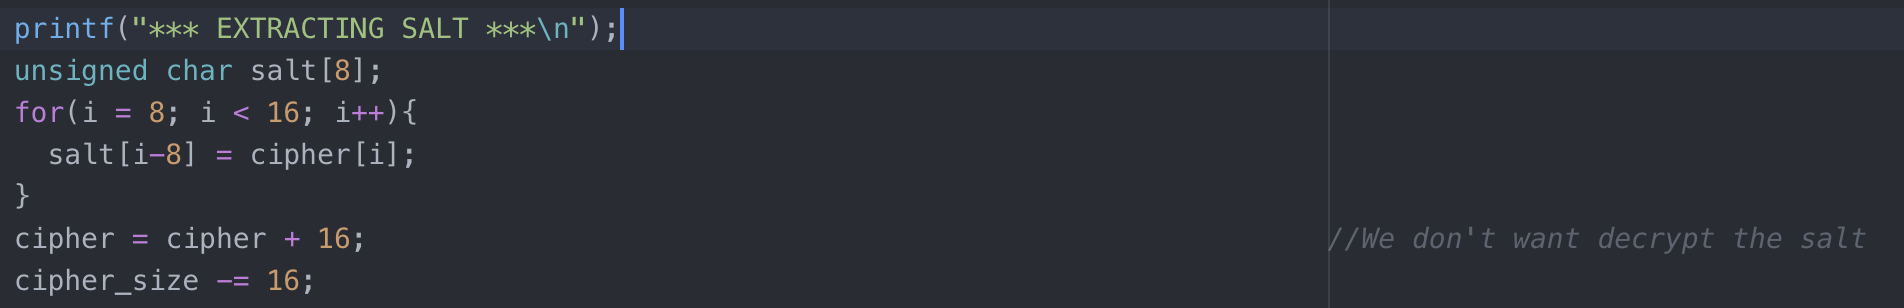
\includegraphics[width=1\textwidth]{pic1-hw2-1635747}
  \label{fig:Salt extraction}
\end{figure}

As we see in the figure after extracting the salt we move the pointer of ciphertext by 16 bytes, this because we don't want decrypt the salt (Remember: in the first 8 bytes we have the string "Salted\_\_", in the second 8 bytes we have the salt)

Now that we have our parameters we are ready to derive the key.

\subsection{PBKDF2 algorithm}
Is a key derivation algorithm with a sliding computational cost, used to reduce vulnerabilities to brute force attacks. It applies a pseudorandom function,  such as hash-based message authentication code (HMAC), to the input password along with a salt value and repeats the process many times to produce a derived key. The added computational work makes password cracking much more difficult, and is known as {\em key stretching}.
The PBKDF2 key derivation function has five input parameters:

\bigskip
$ DK = PBKDF2(PRF, Password, Salt, iter, dkLen) $
\bigskip

where the only parameter we don't know is PRF that is the pseudorandom function applied. OpenSSL use HMAC with sha256 digest as default. This is why it was important to study the default parameters, without these in our code we could not have applied the pbkdf2 function. In C we have implemented pbkdf2 as follow:

\begin{figure}[!ht]
  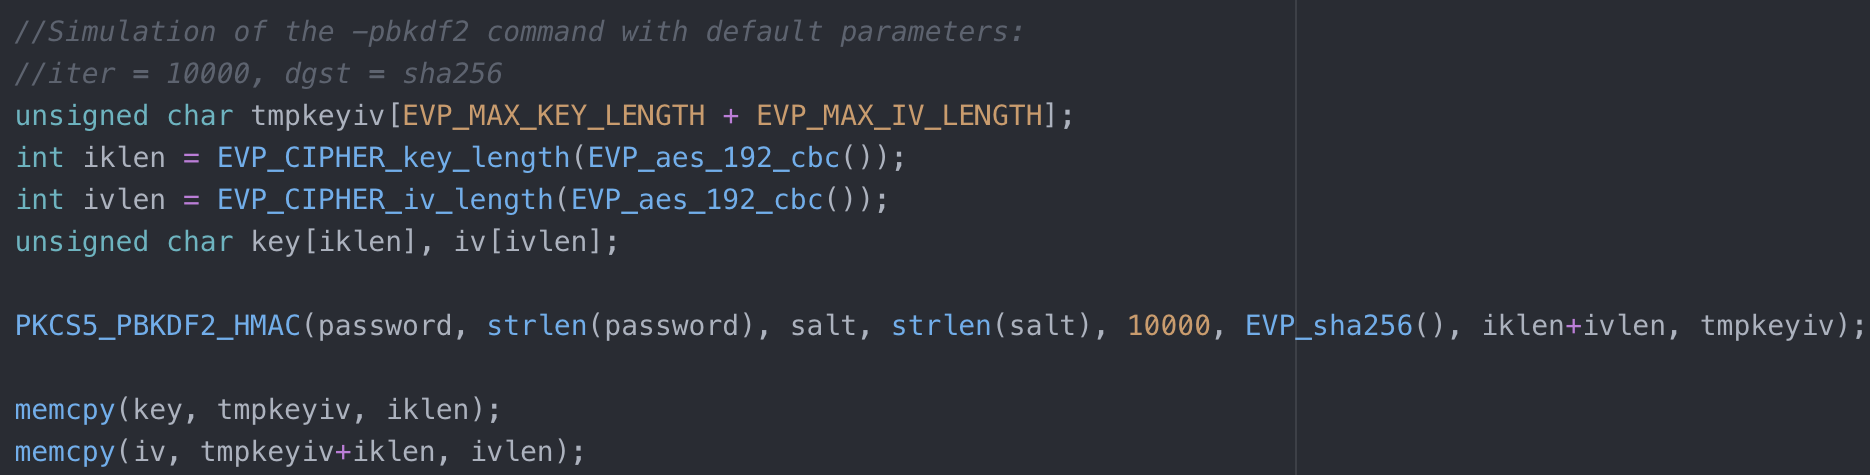
\includegraphics[width=1\textwidth]{pic2-hw2-1635747}
  \label{fig:pbkdf2 implementation}
\end{figure}
\newpage

We took this function directly from the openssl documentation. Note that we did not talk about the initialization vector, but we just need to know that if it is not specified this is generated together with the key.

\subsection{Plaintext Checking}
Another important thing that we know is that the original plaintext is an {\em english} text and the encryption password is a {\em meaningful english word}. This two data is very important because reduce our dictionaries research, in fact all we need is a basic english dictionary.

Said that, once the file has been decrypted we have to check the result. For doing tihs we use two tests: first, if openssl returns a {\em bad decrypt} error in the decryption, then we discard that word, otherwise we take the resulting plaintext and check if it is ascii. In code we have a function called {\em decrypt} that return -1 if there was an error, then we have a function that return 1 if plaintext is ascii, 0 otherwise.

\begin{figure}[!ht]
  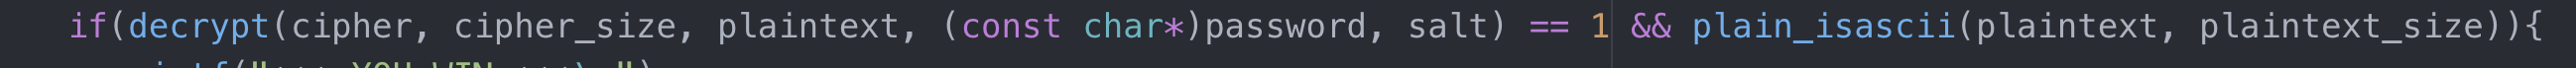
\includegraphics[width=1\textwidth]{pic3-hw2-1635747}
  \label{fig:Ascii check}
\end{figure}

\subsection{Chosen Dictionary}
For our attack we test two different dictionary. The first contains 84000 ordered words from

http://www.gwicks.net/dictionaries.htm \newline and the second contains 10000 ordered words from

https://www.mit.edu/~ecprice/wordlist.10000.

Then for analyze the result we report the time for decrypting and the time in the worst case.

\section{Experimentation}
\begin{figure}[!ht]
  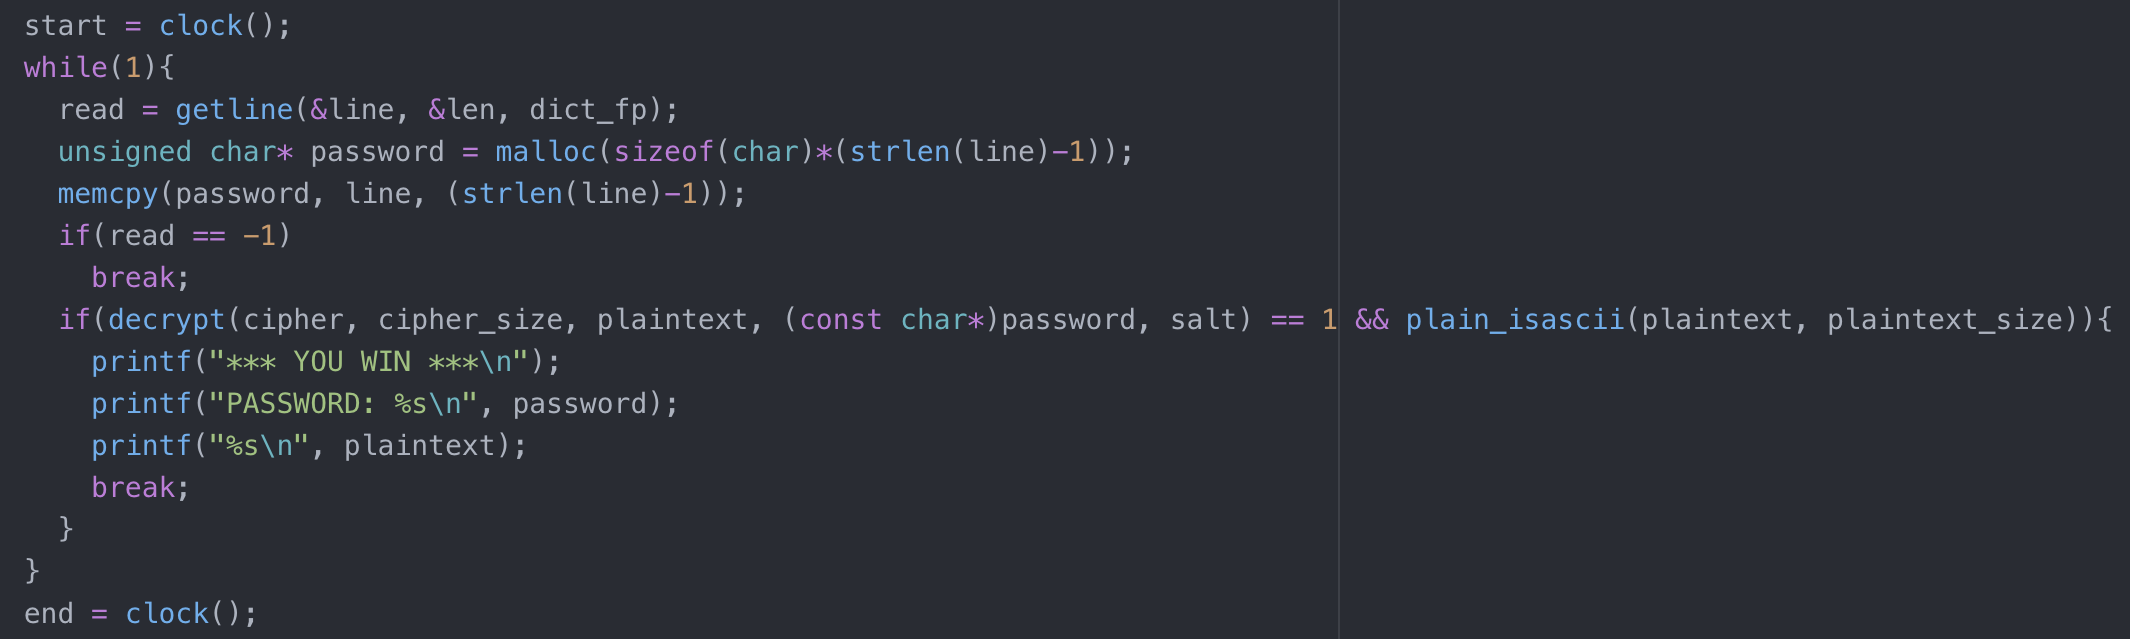
\includegraphics[width=1\textwidth]{pic4-hw2-1635747}
  \label{fig:Dictionary attack}
\end{figure}

This is our dictionary attack. Simply it reads line by line the dictionary, discard the newline char, and check if it is the right password, then print the plaintext.

The right password is: {\em learning}

and the plain text is:
\begin{quote}
To be, or not to be: that is the question:
Whether 'tis nobler in the mind to suffer
The slings and arrows of outrageous fortune,
Or to take arms against a sea of troubles,
And by opposing end them? To die: to sleep;
No more; and by a sleep to say we end
The heart-ache and the thousand natural shocks
That flesh is heir to, 'tis a consummation
Devoutly to be wish'd. To die, to sleep;
To sleep: perchance to dream: ay, there's the rub;
For in that sleep of death what dreams may come
When we have shuffled off this mortal coil,
Must give us pause: there's the respect
That makes calamity of so long life;
For who would bear the whips and scorns of time,
The oppressor's wrong, the proud man's contumely,
The pangs of despised love, the law's delay,
The insolence of office and the spurns
That patient merit of the unworthy takes,
When he himself might his quietus make
With a bare bodkin? who would fardels bear,
To grunt and sweat under a weary life,
But that the dread of something after death,
The undiscover'd country from whose bourn
No traveller returns, puzzles the will
And makes us rather bear those ills we have
Than fly to others that we know not of?
Thus conscience does make cowards of us all;
And thus the native hue of resolution
Is sicklied o'er with the pale cast of thought,
And enterprises of great pith and moment
With this regard their currents turn awry,
And lose the name of action.--Soft you now!
The fair Ophelia! Nymph, in thy orisons
Be all my sins remember'd.
\end{quote}

As a first attempt we tries with the dictionary of 84000 words and to get right password and relatively plaintext it takes 514.127709 seconds, about 9 minutes. This means that in the worst case where the alghorithm has to scan all the words it take about 18 minutes, because the right password is just after the half.

Instead with the dictionary of 10000 words we are still arriving at the right result with 61.469973 seconds, about 1 minute and in the worst case it takes 2 minutes. This is a very nice result. Now we are ready to draw our conclusions.

\section{Conclusion}
This experiment tells us that encrypting a message with a common password is almost useless because even a simple algorithm like this can decrypt it and find the password in about 2 minutes.

The algorithm presented is really very simple and specific for the preliminary data we had, but it is enough to think that putting a char non ascii at the beginning of the plaintext this algorithm would never reach the right solution. However in most cases when we exchange messages we don't care about these details, but we only enter a password. So it's important to always try to enter a password that is never a common word.

About the algorithm time we have seen that this depends on the chosen dictionary, in this case even a small dictionary of 10000 words returns the right result. In other problems we could be dealing with dictionaries that could exceed even a million words, in this case the algorithm could be improved by splitting the dictionary into several parts and parallelizing the execution.

\begin{thebibliography}{99}

\bibitem{wiki}
{\em PBKDF2 - Wikipedia}.
  \verb|https://en.wikipedia.org/wiki/PBKDF2|

\bibitem{wiki}
{\em Dictionary Attack - Wikipedia}.
  \verb|https://en.wikipedia.org/wiki/Dictionary_attack|

\bibitem{link}
OpenSSL Documentation.
\verb|https://www.openssl.org/docs/manmaster/man3/|

\bibitem{link}
OpenSSL GitHub Repository.
\verb|https://github.com/openssl/openssl|

\end{thebibliography}

\end{document}
